% Copyright 2004 by Till Tantau <tantau@users.sourceforge.net>.
%
% In principle, this file can be redistributed and/or modified under
% the terms of the GNU Public License, version 2.
%
% However, this file is supposed to be a template to be modified
% for your own needs. For this reason, if you use this file as a
% template and not specifically distribute it as part of a another
% package/program, I grant the extra permission to freely copy and
% modify this file as you see fit and even to delete this copyright
% notice. 

\documentclass{beamer}[10pt]
%\usepackage{graphicx}

\graphicspath{ {../Animations/LargePlate/4000/}{../Animations/Plate/Plate20/}{../Plots/}{../Animations/LargePlate/8000/} }
\usepackage{hyperref}
% There are many different themes available for Beamer. A comprehensive
% list with examples is given here:
% http://deic.uab.es/~iblanes/beamer_gallery/index_by_theme.html
% You can uncomment the themes below if you would like to use a different
% one:
%\usetheme{AnnArbor}
%\usetheme{Antibes}
%\usetheme{Bergen}
%\usetheme{Berkeley}
%\usetheme{Berlin}
%\usetheme{Boadilla}
%\usetheme{boxes}
%\usetheme{CambridgeUS}
%\usetheme{Copenhagen}
%\usetheme{Darmstadt}
%\usetheme{default}
%\usetheme{Frankfurt}
%\usetheme{Goettingen}
%\usetheme{Hannover}
%\usetheme{Ilmenau}
%\usetheme{JuanLesPins}
%\usetheme{Luebeck}
\usetheme{Madrid}
%\usetheme{Malmoe}
%\usetheme{Marburg}
%\usetheme{Montpellier}
%\usetheme{PaloAlto}
%\usetheme{Pittsburgh}
%\usetheme{Rochester}
%\usetheme{Singapore}
%\usetheme{Szeged}
%\usetheme{Warsaw}

\title{TMA4220 - PDEs /w FEM}

% A subtitle is optional and this may be deleted
\subtitle{Programming Project}

\author{G.~A.~Hasle \and T.~Baerland \and E.~Ingebrigtsen}
% - Give the names in the same order as the appear in the paper.
% - Use the \inst{?} command only if the authors have different
%   affiliation.

%\institute[Universities of Somewhere and Elsewhere] % (optional, but mostly needed)
%{
%  \inst{1}%
%  Department of Computer Science\\
%  University of Somewhere
%  \and
%  \inst{2}%
%  Department of Theoretical Philosophy\\
%  University of Elsewhere}
% - Use the \inst command only if there are several affiliations.
% - Keep it simple, no one is interested in your street address.

\date{FEM on Free Vibrations}
% - Either use conference name or its abbreviation.
% - Not really informative to the audience, more for people (including
%   yourself) who are reading the slides online

\subject{Theoretical Computer Science}
% This is only inserted into the PDF information catalog. Can be left
% out. 

% If you have a file called "university-logo-filename.xxx", where xxx
% is a graphic format that can be processed by latex or pdflatex,
% resp., then you can add a logo as follows:

% \pgfdeclareimage[height=0.5cm]{university-logo}{university-logo-filename}
% \logo{\pgfuseimage{university-logo}}

% Delete this, if you do not want the table of contents to pop up at
% the beginning of each subsection:


% Let's get started
\begin{document}

\begin{frame}
  \titlepage
\end{frame}

% Section and subsections will appear in the presentation overview
% and table of contents.
\section{Presentation}

\subsection{Introduction}
\begin{frame}{Introduction}
  \begin{itemize}
  \begin{block}{The Free Vibration Equation}
\begin{equation}
\rho\frac{\partial^2u}{\partial t^2} = \nabla\sigma(u)
\label{eq:Free Vibration}
\end{equation}
\end{block}
  \item {   
    Is it possible to model 
    \begin{figure}
    \centering
    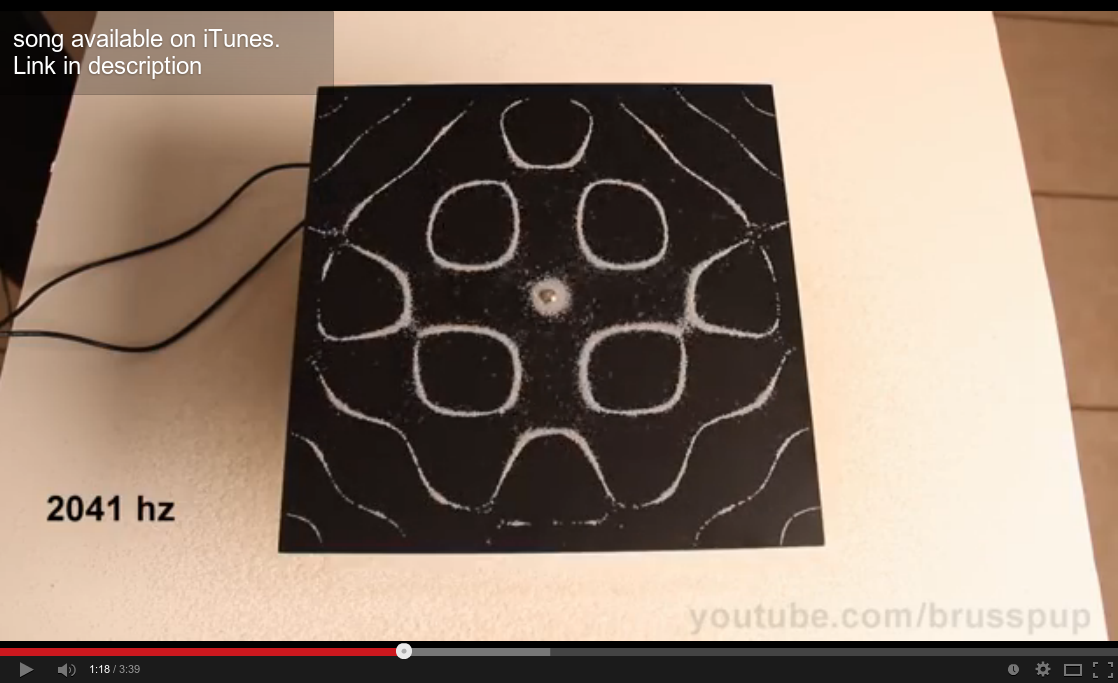
\includegraphics[scale=0.1]{yosnap.png}
    \end{figure}
	with Finite Element Methods?  
  }
  % You can also specify when the content should appear
  % by using <n->:
  \end{itemize}
\end{frame}

\begin{frame}{Introduction}	
\begin{itemize}
\item {
We want a variational formulation of (\ref{eq:Free Vibration})

}
\item {
Usual procedure: Multiply (\ref{eq:Free Vibration}) with a test function $v$ and integrate over the domain to obtain 
\begin{equation}
\rho \int\limits_{\Omega} \ddot{u}\cdot v\mathrm{d}\Omega = - \int\limits_{\Omega}\epsilon\left(v\right)\cdot C \epsilon\left(u\right)\mathrm{d}\Omega
\label{eq:Variational Form}
\end{equation}
}
\end{itemize}
\end{frame}

\begin{frame}{Introduction}


  \begin{itemize}
  \item {
    Semi-discretization on (\ref{eq:Variational Form}) yields
    \begin{equation}
    M\ddot{\boldsymbol{u}} = -A\boldsymbol{u}
    \label{eq:free vib, linear sys}
    \end{equation}
    \footnotesize
    \begin{align*}
    A  = \left[ A_{ij} \right] & = \int\limits_{\Omega} \varepsilon \left( \varphi_i \right)^T C\varepsilon\left( \varphi_j \right) \mathrm{d} \Omega \\
    M  = \left[ M_{ij} \right] &= \int\limits_{\Omega} \ \rho \varphi_{i}^T \varphi_j \mathrm{d} \Omega \\ 
    \end{align*}
    \normalsize
  }
  \item {
	Assuming $\boldsymbol{u} = \boldsymbol{u}e^{i\omega t}$ on (\ref{eq:free vib, linear sys}) yields the generalized eigenvalue problem
	\begin{equation}
	\omega^2 M\boldsymbol{u} = A\boldsymbol{u}
	\label{eq:eigenvalue problem}
	\end{equation}	  
  }
  \end{itemize}
\end{frame}

\begin{frame}{Building $A$ and $M$}
\centering
\begin{equation*}
\varphi_{\hat{i},1} = \begin{bmatrix}
\varphi_{\hat{i}} \\ 0 \\ 0
\end{bmatrix}, \quad
\varphi_{\hat{i},2} = \begin{bmatrix}
 0 \\ \varphi_{\hat{i}}\\ 0
\end{bmatrix}, \quad
\varphi_{\hat{i},3} = \begin{bmatrix}
0 \\ 0 \\ \varphi_{\hat{i}}
\end{bmatrix}.
\end{equation*}
$\varphi_{\hat{i}}\big|_{T_k} = c_0 + c_1x+c_2y + c_3z$
\begin{equation*}
\boldsymbol{\varepsilon}\left(\varphi_{\hat{i},d}\right) = \begin{bmatrix}
c_1 \\ 0 \\ 0 \\ c_2 \\c_3 \\ 0
\end{bmatrix}
, \begin{bmatrix}
0 \\ c_2 \\ 0 \\ c_1 \\ 0 \\ c_3 \end{bmatrix},
\begin{bmatrix}
0 \\ 0 \\ c_3 \\ 0 \\ c_1 \\ c_2 \end{bmatrix}
\end{equation*}
\end{frame}
\begin{frame}{Building $A$ and $M$}
\begin{itemize}
\item {
Stiffness matrix $A$:
\begin{equation*}
    \varepsilon\left( \varphi_i \right)^T C\varepsilon\left( \varphi_j \right) \mathrm{area}(T_k)
\end{equation*}}
\item {
Mass matrix $M$:
\begin{equation*}
 \rho\cdot \text{det}(B)M^P_{\alpha,\beta}
\end{equation*}
}
\end{itemize}
\end{frame}
\begin{frame}{Implementation}
\begin{itemize}
\item {Solve $	\omega^2 M\boldsymbol{u} = A\boldsymbol{u}$ for the $k$ lowest eigenvalues using \textsc{Matlab}'s \texttt{eigs}}
\item {Use the different eivenvectors $\boldsymbol{u_i}$ to make animations}
\item {$\boldsymbol{x}=\boldsymbol{x_0}+\alpha \boldsymbol{u_i}\sin(t)$}
\item {Collection of \textsc{Matlab} scripts/functions}
\item {Open to different geometries (chess pawn, gun, plate) and materials}
\item {ParaView for the post processing}
\end{itemize}
\end{frame}

\begin{frame}{Animations}
\begin{itemize}
\item{
\href{http://www.youtube.com/watch?v=yc8ZH4cEz5g&feature=youtu.be}{\beamergotobutton{Animation of a gun(!). Mode 7,9,10 and 20}}
}
\item{
\href{http://www.youtube.com/watch?v=zDAihCeC7Oo&feature=youtu.be}{\beamergotobutton{Animation of a chess pawn. Mode 7,10,14 and 15}}
}
\end{itemize}
\end{frame}

\begin{frame}{Boundary condition}
\centering
Can we have boundary conditions?
\vspace*{2em}
  \begin{columns}[T]
    \begin{column}{.5\textwidth}
    \begin{itemize}
    		\item {Physical interpretation}
		\item {Free vibration}
		\item {Can use Dirichlet}
		\item{
\href{http://www.youtube.com/watch?v=PGEh8rN9Qeo&feature=youtu.be}{Animation of a chess pawn. Homogeneous boundary conditions}
}
	\end{itemize}
    \end{column}
    \begin{column}{.5\textwidth}
    \begin{figure}
    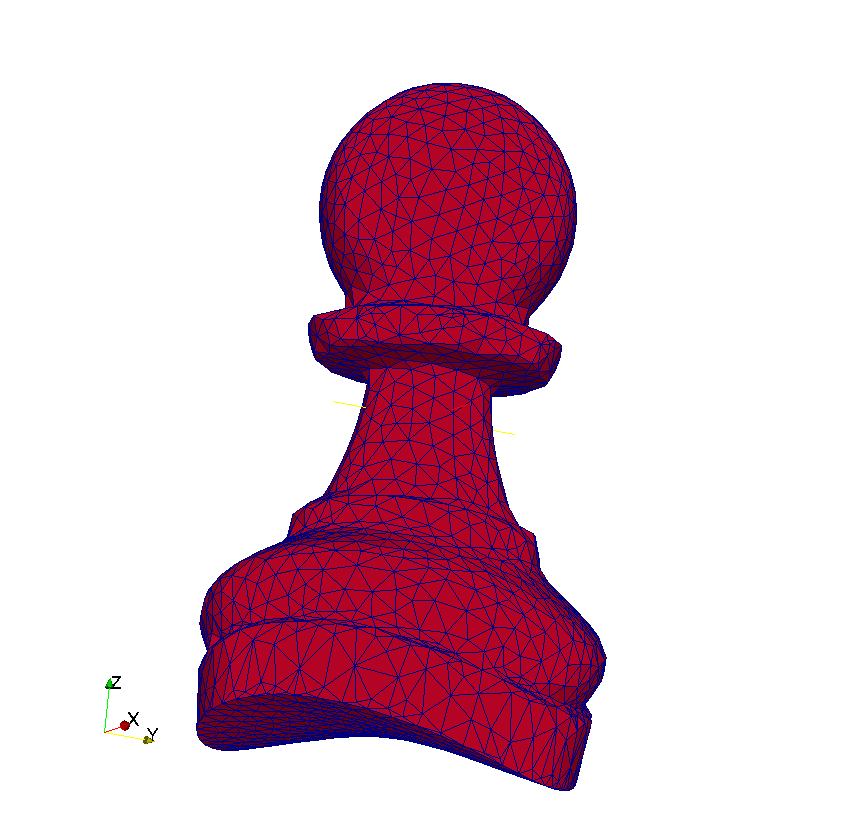
\includegraphics[width=0.7\textwidth>]{PawnMode15.png}    
    \end{figure}
    \end{column}
  \end{columns}
\end{frame}

\begin{frame}{Back to the plate}
\begin{itemize}
\item { An example of our results (3443 Hz):
\begin{figure}
\centering
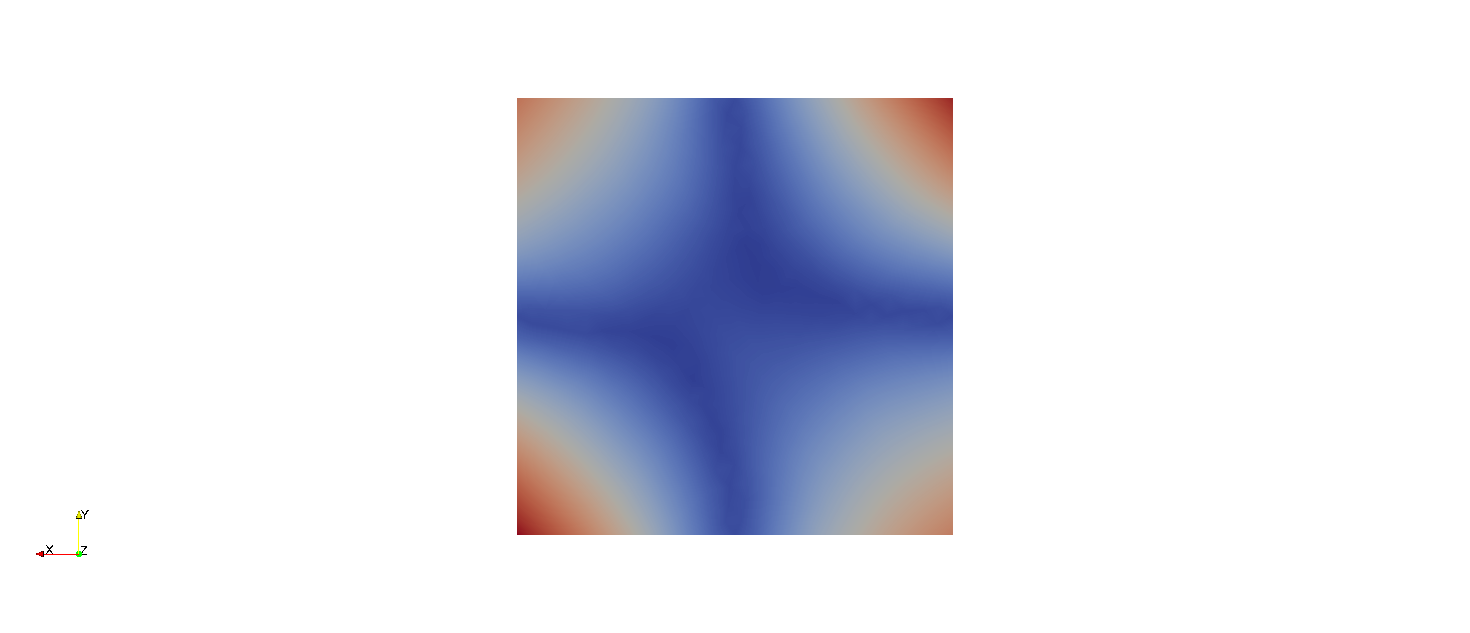
\includegraphics[scale=0.3, trim= 100mm 0mm 100mm 0mm, clip]{1small.png}
\end{figure}}
\item{Needs finer mesh}
\end{itemize}

\end{frame}

\begin{frame}{Back to the plate (cont.)}
\begin{itemize}
\item {
Finer mesh gives (3031.6 Hz):
\begin{figure}
\centering
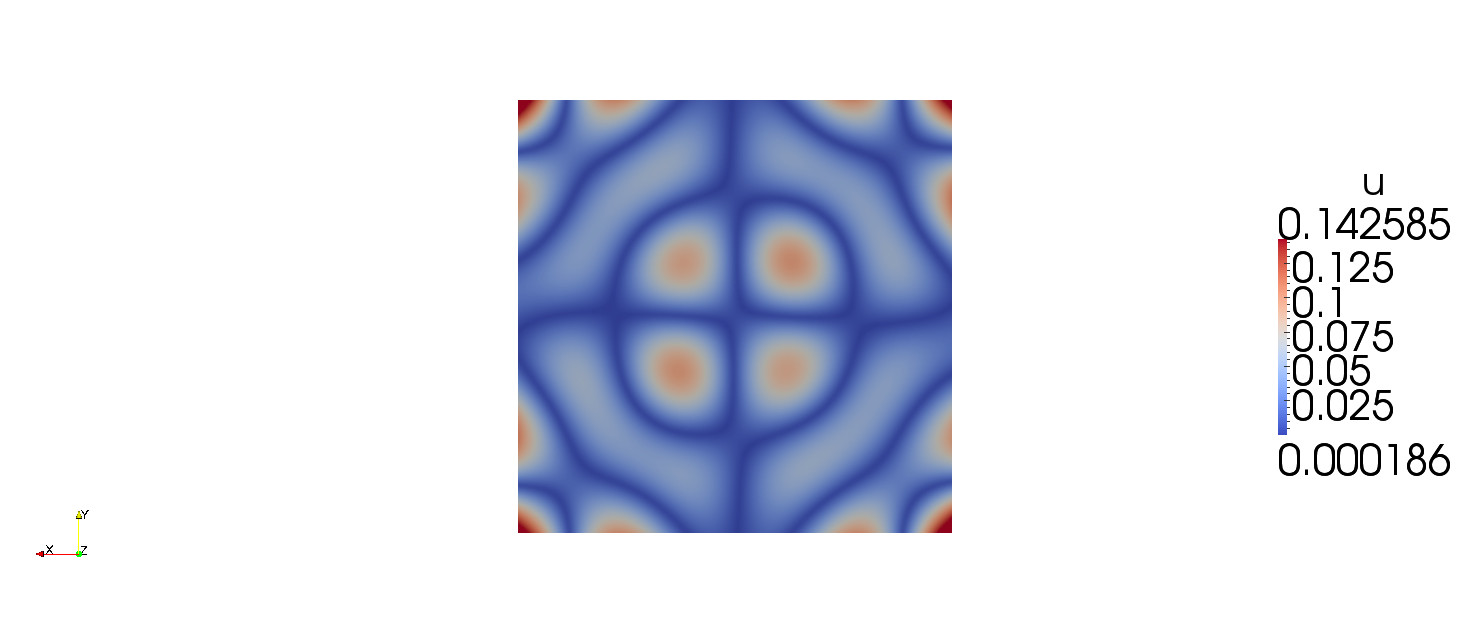
\includegraphics[scale=0.3, trim= 100mm 0mm 100mm 0mm, clip]{18.png}
\end{figure}
}
\item {Picks up frequencies closer together.}
\end{itemize}

\end{frame}



\begin{frame}{Even more plates}
\begin{itemize}
\item{
7207Hz
\begin{figure}
\centering
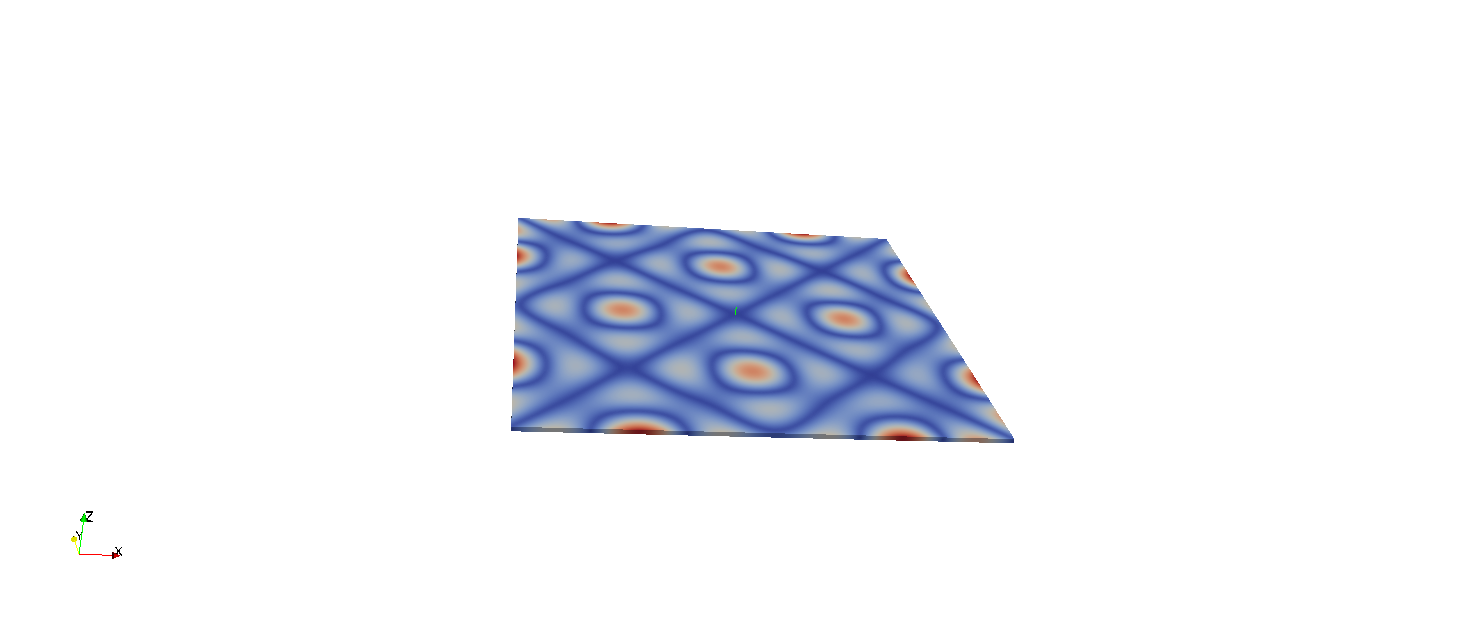
\includegraphics[scale=0.3, trim= 100mm 0mm 100mm 0mm, clip]{13angle.png}
\end{figure}

}
\end{itemize}
\end{frame}

\begin{frame}{Even more plates}
\begin{itemize}
\item{
7222Hz
\begin{figure}
\centering
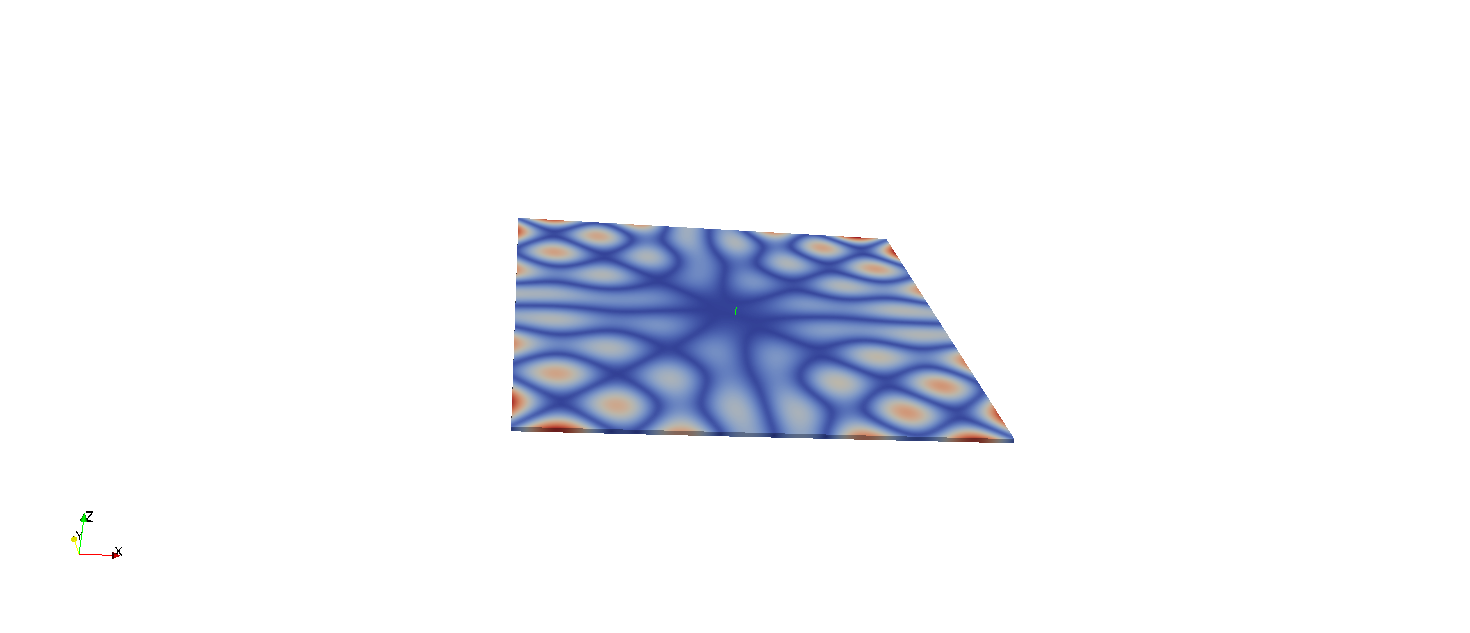
\includegraphics[scale=0.3, trim= 100mm 0mm 100mm 0mm, clip]{12a.png}
\end{figure}

}
\end{itemize}
\end{frame}

\begin{frame}{Even more plates}
\begin{itemize}
\item{
7261Hz
\begin{figure}
\centering
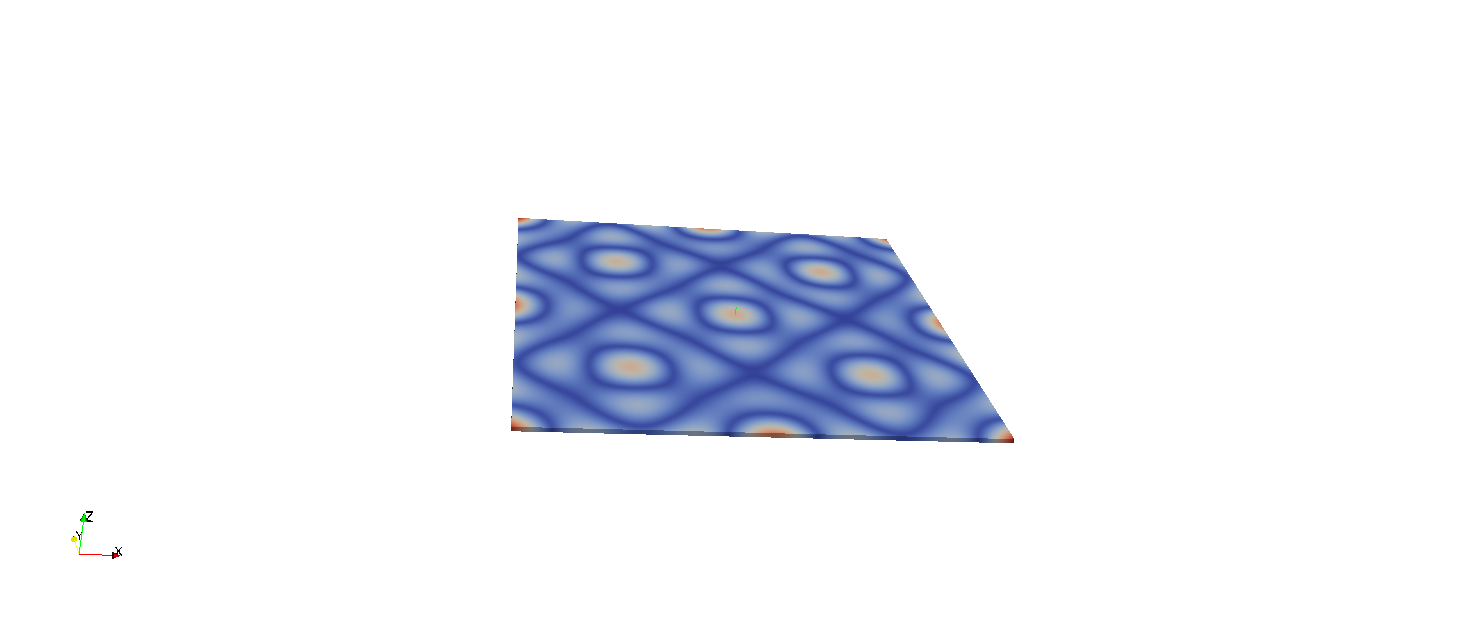
\includegraphics[scale=0.3, trim= 100mm 0mm 100mm 0mm, clip]{11a.png}
\end{figure}

}
\end{itemize}
\end{frame}

\begin{frame}{Even more plates}
\begin{itemize}
\item{
7282Hz
\begin{figure}
\centering
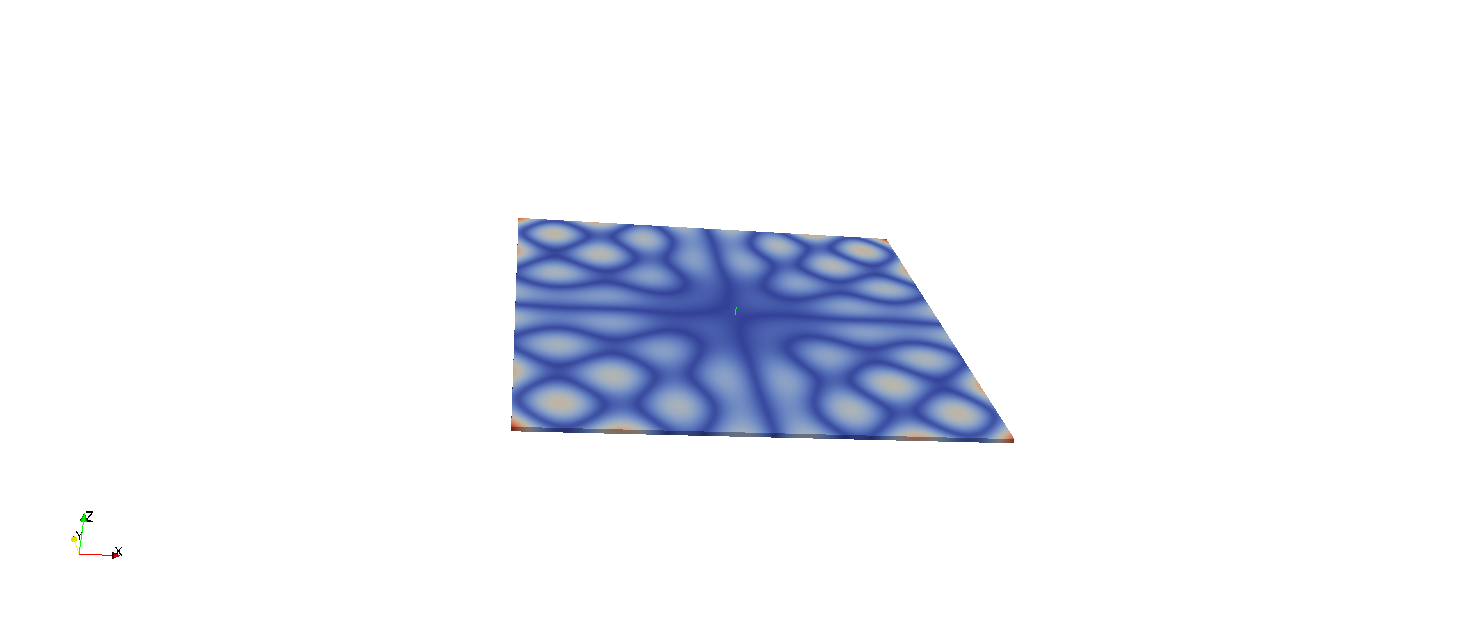
\includegraphics[scale=0.3, trim= 100mm 0mm 100mm 0mm, clip]{10a.png}
\end{figure}

}
\end{itemize}
\end{frame}

\begin{frame}{Even more plates}
\begin{itemize}
\item{
7797Hz
\begin{figure}
\centering
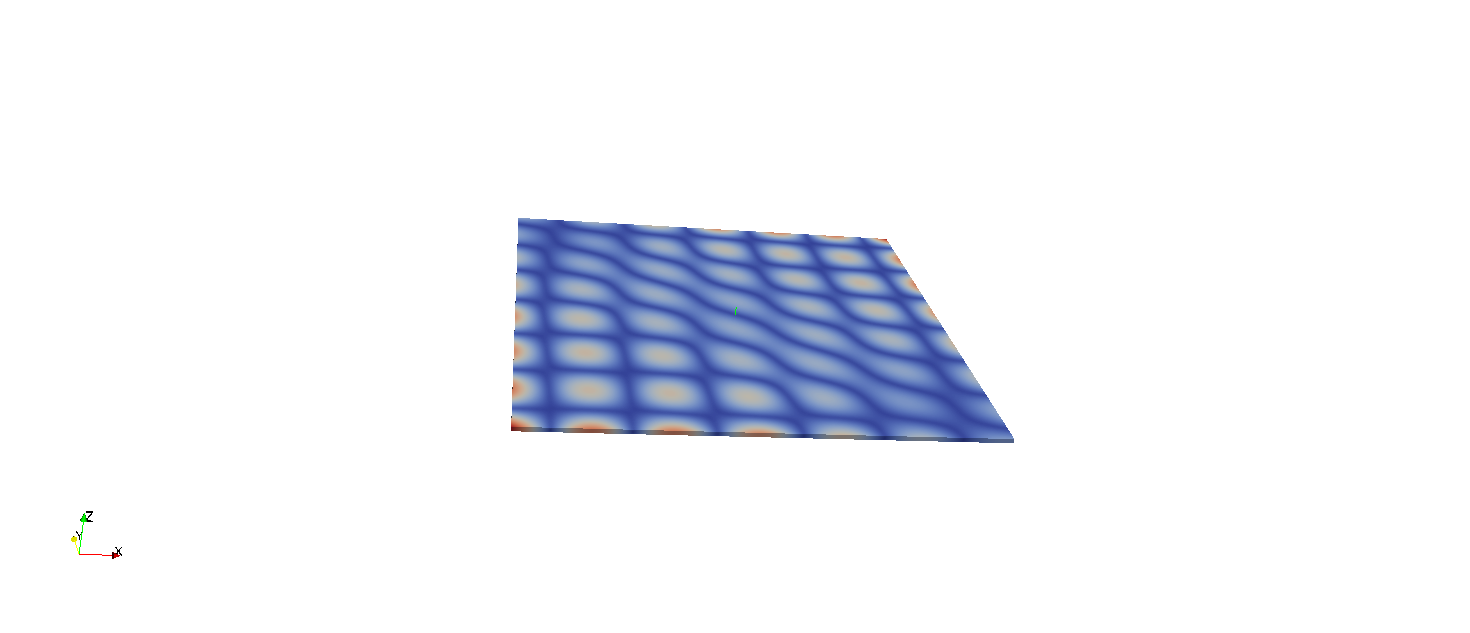
\includegraphics[scale=0.3, trim= 100mm 0mm 100mm 0mm, clip]{7a.png}
\end{figure}

}
\end{itemize}
\end{frame}


\begin{frame}{Even more plates}
\begin{itemize}
\item{
8049HZ
\begin{figure}
\centering
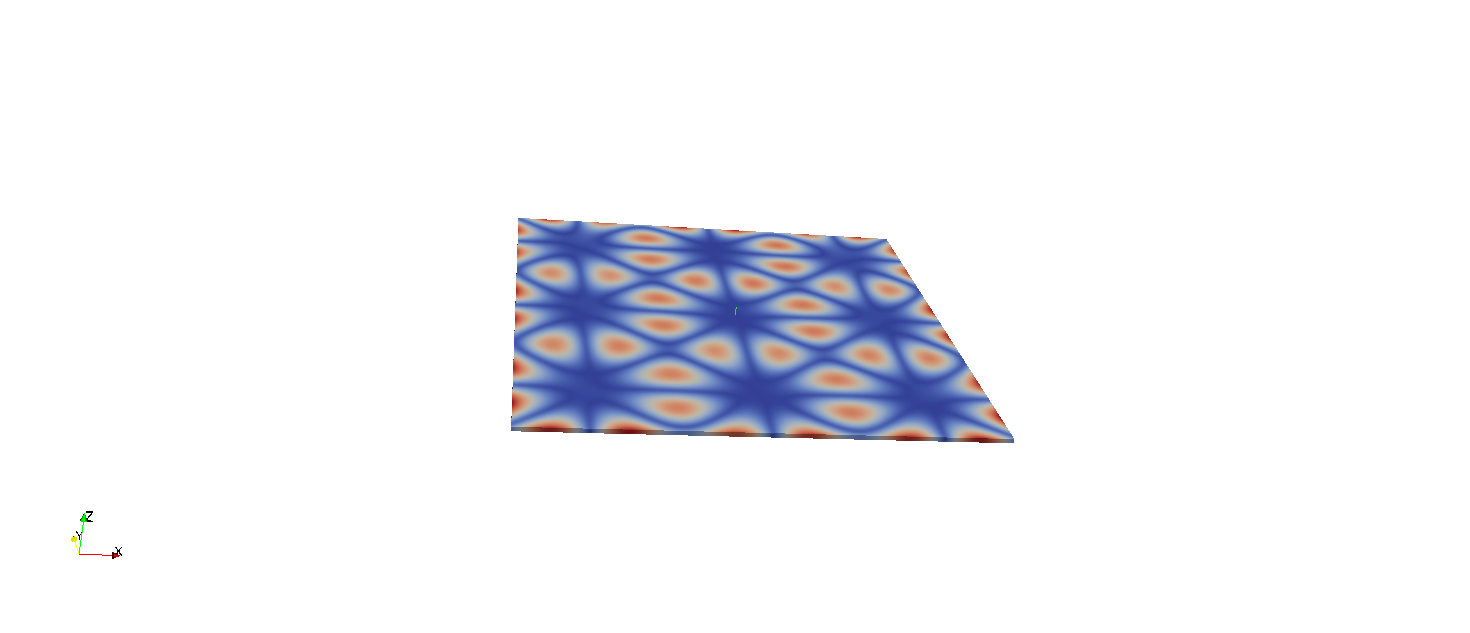
\includegraphics[scale=0.3, trim= 100mm 0mm 100mm 0mm, clip]{1a.png}
\end{figure}

}
\end{itemize}
\end{frame}


\begin{frame}{Even more plates}
\begin{itemize}
\item{
8121Hz
\begin{figure}
\centering
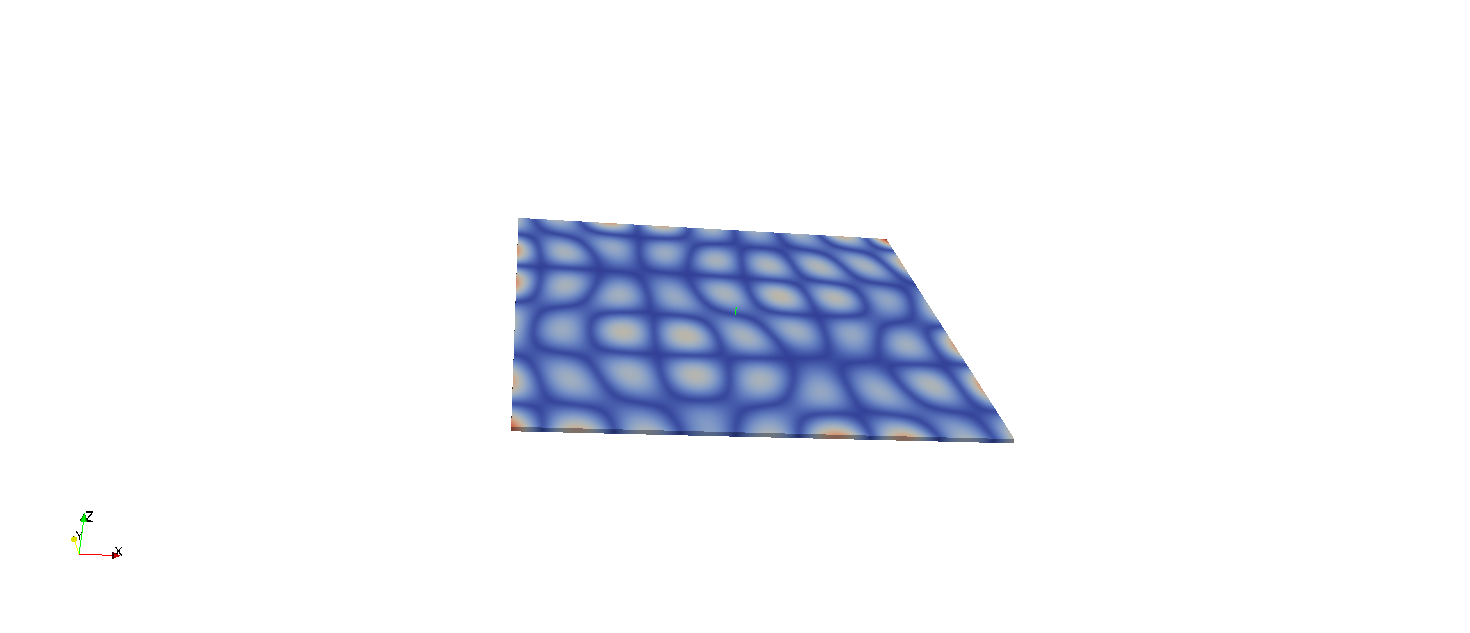
\includegraphics[scale=0.3, trim= 100mm 0mm 100mm 0mm, clip]{5a.png}
\end{figure}

}
\end{itemize}
\end{frame}










\end{document}



